\chapter{Evaluation}
\label{chapter:evaluation}

In order to be worthwhile, skip regex must be faster than standard
regex and there must be ample opportunity to apply them. To evaluate
the degree to which skip regex meet these goals, we perform a number
of experiments.  We present a series of micro benchmarks to demonstrate
the performance of skip regex under specific conditions. The micro
benchmarks show that the performance of skip regex is
at least as good as the equivalent standard regex execution, and 
is often significantly better. To determine the usefulness of skip
regex for regular expressions found in the wild, we scraped
\verb'crates.io', the Rust package repository,
for regular expressions and tested to see how applicable each of the 
optimizations we perform are. Finally, we perform a case study walking
through the steps a programmer might take while parsing logs from
an Apache Kafka instance.

\section{Microbenchmarks}

Microbenchmarks alone are not typically enough to develop a high
level understanding of application performance, yet they remain
quite useful for demonstrating performance edge cases. Put another
way, microbenchmarks are excellent tools for performance story
telling. Sometimes such story telling can be used to deceive,
but we will attempt to avoid any deception and instead focus
on the performance trade-offs of skip regex.

% TODO: explain methodology.
The micro benchmarks we present in this section each consist of
a regex template and an input template which get instantiated
based off of some scaling factor and then run with different
backends. The scaling factor typically increases the input
size by a constant number of characters, and less commonly
increases the regex size. We run each microbenchmark at a
number of different scaling factors using Rust's built in
benchmarking facility, which takes a number of samples before
reporting the average runtime plus the spread between the minimum
and maximum runtime. We indicate the spread by attaching error bars to
each datapoint in our scatter plots.

In order to demonstrate the utility of different optimizations,
we execute the benchmarks with different engines and different
optimizations enabled. The standard regex engines are called
\texttt{baseline\allowbreak -\allowbreak backtrack} and
\texttt{baseline\allowbreak -\allowbreak pike}, while the
skip backends are called \texttt{skip\allowbreak -\allowbreak backtrack}
and \texttt{skip\allowbreak -\allowbreak pike},
with a number of optimization specifiers tacked onto the end to
indicate which optimizations have been enabled. For example,
\texttt{skip\allowbreak -\allowbreak backtrack\allowbreak -\allowbreak
        ds\allowbreak -\allowbreak es\allowbreak -\allowbreak sl}
indicates that the skip backtracker with $.*$ scanning, $e*$ scanning,
and literal skipping enabled.

% TODO: open up a documentation PR so that other people don't
%       have to go digging through rustc source to figure out
%       what the +/- means.

\subsection{Best Possible Case: A Big Skip}

The best possible case for skip regex is where a regex is composed
entirely of large literals. In such a case a standard regex engine
must laboriously test ever input character, while a skip regex
engine is allowed to traverse the input in a few big hops. Figure
\ref{fig:a:big:skip} illustrates just such a case. Here we executed the
regex \verb'/aaaa(bbbb)cccc/' on an input of the form \verb'aaaabbbbcccc'.
In both the regex and the input, the number of \verb'a' and \verb'c'
characters was multiplied by the scaling factor. As we might expect,
the graph shows that both the skip Pike VM and the skip backtracker
beat out the non-skip backtracker quite handily, with the running time
of the skip engines remaining virtually flat as the running
time of the standard backtracker grows linearly with the scaling factor.
The performance improvement is entirely due to the literal skip
optimization, as shown by the fact that the performance of the skip
backtracker with literal skipping disabled matches the
\verb'baseline-backtrack' configuration.

\begin{figure}
\label{fig:a:big:skip}
\caption{A Big Skip}

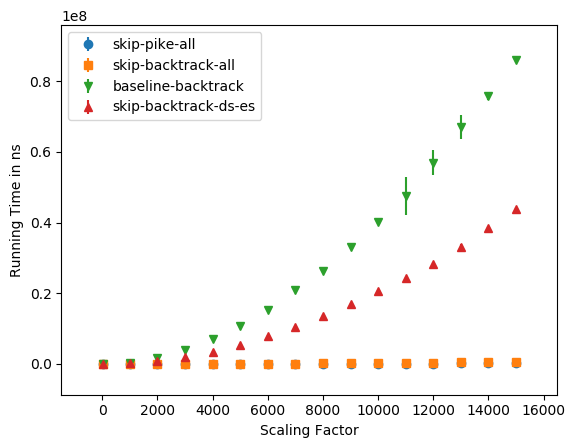
\includegraphics{resources/a-big-skip.png}
\end{figure}

\subsection{Leading $.*$}

While not quite as good as being able to traverse the whole input
in a few hops, a leading $.*$ which can be scanned over to find the
correct terminator after the first try is still very fast. A standard
regex must go through the expensive process of spawning two new threads
for each character of input, one of which will die after each step.
By contrast, a skip regex engine can drop right into a fast substring
search algorithm. We produced figure \ref{fig:leading:dotstar} by executing
\verb'/.*(aaaa)/' on \verb'baaaa' with \verb'b' repeated according
to the scaling factor. The graph shows that all the engines are linear
in the size of the input, but the constant factor for the skip engines
is so much lower that they appear nearly constant time.

\begin{figure}
\caption{Leading $.*$}
\label{fig:leading:dotstar}

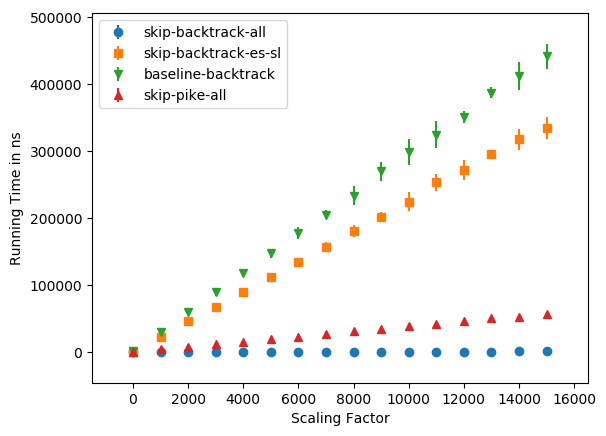
\includegraphics{resources/leading-dotstar.png}
\end{figure}

\subsection{$.*$ Bounce}

It would not be fair to showcase the best possible case for the
$.*$ scan optimization without also demonstrating the worst
case. If the literal terminator appears many times before the
end of the repetition, the skip engine will be forced to
rapidly enter and leave the substring search algorithm, spawning
two new threads on every iteration. This essentially makes
the dotstar scan optimized code no better than a standard regex
execution. To demonstrate this worst case situation we executed
the regex \verb'/.*a(bbbb)/' on \verb'cabbbb' with \verb'ca'
repeated according to the scaling factor. Figure \ref{fig:dotstar:bounce}
shows that the skip backtracker is slower than the standard
backtracker due to the overhead of switching back and forth between the
literal searcher and main engine loop. When the $.*$ optimization is
turned off, the skip backtracker behaves just like the standard
backtracker. This example was constructed to showcase the worst
case for the $.*$ scan optimization, but it seems less likely to appear
in the wild than the best case.

\begin{figure}
\caption{$.*$ Bounce}
\label{fig:dotstar:bounce}

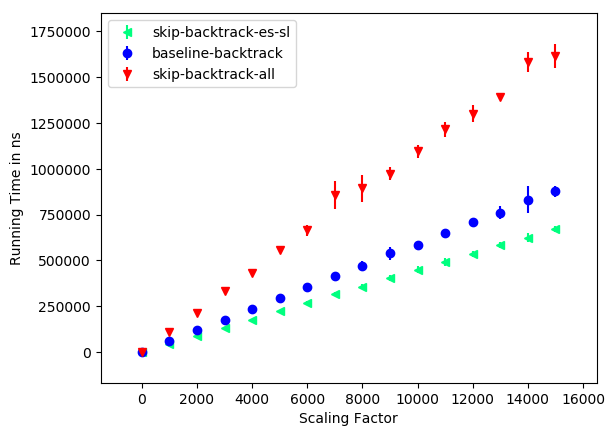
\includegraphics{resources/dotstar-bounce.png}
\end{figure}

\subsection{Leading $e*$ scan}

The other scan optimization only really has a best case, because
the scan is always guaranteed to find the literal terminator. The
effectiveness of the optimization is entirely determined by the
size of the input, something which can be completely described
by one experiment. We produced figure \ref{fig:leading:noncontaining:estar}
by executing the regex \verb'a*foo(bar)' on \verb'afoobar' with \verb'a'
repeated according to the scaling factor. Just as in the ``Leading $.*$''
experiment, all engines are linear, but the skip backends are so much
faster that they appear almost constant time.

\begin{figure}
\caption{Leading $e*$}
\label{fig:leading:noncontaining:estar}

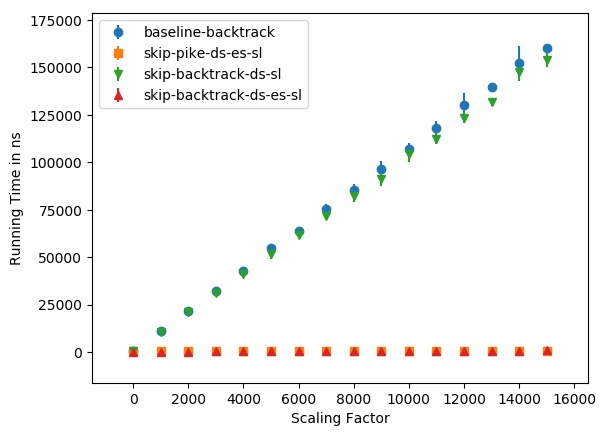
\includegraphics{resources/leading-noncontaining-estar.png}
\end{figure}

\subsection{No Opt}

In some cases no optimizations can be usefully applied to a skip
regex. We include such a case to demonstrate that with the exception
of a bouncing $.*$ optimization, the performance of skip regex is
no worse than that of standard regex. We produced figure 
\ref{fig:justtwo:branch}
by executing the regex \verb'/(ab|ac)*/' on \verb'ab' with
the input multiplied by the scaling factor. The fact that the
two branches of the alternative have intersecting first sets
(in particular $\{a\}$ and $\{a\}$), means that skip optimizations
can't be applied, and there is no clever way to get out of
executing the full kleene star. There is still some spread between
the different engines, most notably between the Pike VMs and the
bactrackers, as backtrackers are generally faster. The skip Pike VM
has a higher constant factor than the standard Pike VM when optimizations
are not helping out because of the increased complexity of its runnable
thread queue. The skip backtracker seems to have a slightly better
constant factor than the standard backtracker for this benchmark.
This difference may come from some slight overhead associated with
unicode support\footnote{Unicode support is turned off for the
standard backtracker in this benchmark, but the code is written
to be generic over both unicode and byte-oriented input, which
may come at a cost.}.

\begin{figure}
\caption{No Opt}
\label{fig:justtwo:branch}

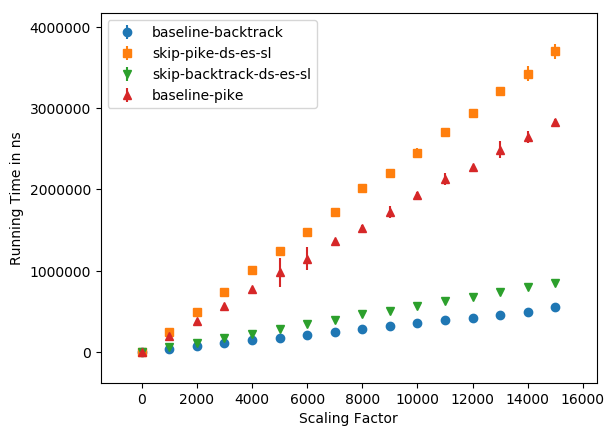
\includegraphics{resources/justtwo-branch.png}
\end{figure}

\section{Log Parsing: A Case Study}

Regular expressions can be used in core application code, but they
are quite frequently used in a more improvisational capacity.
Searching through source code in an editor, filtering and parsing
the output of a previous command in a unix pipeline, and aiding
the construction of quick one-off scripts are all examples of
common use cases for regular expressions. We present an example
walking through the use of skip regex in pre-validated mode
to scrape an Apache Kafka debug log file. This case study
demonstrates the utility of skip regex beyond the library context
illuminated by the \verb'crates.io' figures presented in section
\ref{section:applicability}.

\subsection{Experimental Setup}

Apache Kafka is a Java-based distributed queuing system with
named event categories called topics consisting of several
queues called partitions. Like many network applications,
Kafka contains extensive and configurable debug logging,
which makes it a good source of test data. We configured
Kafka to log as promiscuously as possible and used a simple
python script to repeatedly publish and consume from a 
\verb'test' topic. We used the resultant log file as input
to our scraping script. To make the input log large enough
to observe a difference in performance, we concatenated the
log to itself several times.

The code for our program can be found at \cite{PailesSkipRegexCaseStudy},
but its usage message is worth including here to make
interpreting the invocations we used for our experiments
easier.

\begin{verbatim}
Usage: scrape [options] <log-file>
       scrape -h

Options:
    -v, --validate  First filter with a DFA, then apply skip regex.
    -a, --append    Summarize the append events.
    -n, --named     Summarize the named events.
    -h, --help      Print this help message.
\end{verbatim}

\subsection{Summarizing Append Events}

When a new message is appended to a Kafka log it notes some
metadata about the message such as its size and the offset to
which it was written in the partition. To get a summary of
the append events that occurred in a particular log we 
determine the minimum and maximum offsets appended to,
as well as the total number of append events and the total
number of bytes written. We used the regex
\verb'^.* with first offset: ([0-9]+).*value=([0-9]+).*$'
to extract the offset and the total number of bytes from append
log lines. When we executed our program in first standard mode
then skip mode we got the following output.

\begin{verbatim}
scrape$ du -h server.log
25M     server.log
scrape$ time ./target/release/scrape -a server.log 
3900/111098 (3.51%) append events
1000 min offset
1299 max offset
58110 total bytes written

real    0m0.128s
user    0m0.117s
sys     0m0.012s
scrape$ time ./target/release/scrape -a -v server.log 
3900/111098 (3.51%) append events
1000 min offset
1299 max offset
58110 total bytes written

real    0m0.097s
user    0m0.091s
sys     0m0.006s
\end{verbatim}

Note that because only 3.51\% of lines matched, most of the time
was spent in the DFA discarding non-matching lines in both cases.
The \verb'0.026' second difference in user time then comes from
the 3900 matching lines. When we stripped away the non-matching
lines to more directly observe the difference in performance
of the two NFA simulations we got the following results.

\begin{verbatim}
scrape$ cat server.log | rg "with first offset:" > appends.log 
scrape$ du -h appends.log 
848K    appends.log
scrape$ time ./target/release/scrape -a server.log 
3900/111098 (3.51%) append events
1000 min offset
1299 max offset
58110 total bytes written

real    0m0.129s
user    0m0.120s
sys     0m0.009s
scrape$ time ./target/release/scrape -v server.log 

real    0m0.029s
user    0m0.022s
sys     0m0.007s
\end{verbatim}

This shows that there is significant difference in the performance
of the NFA simulations, and highlights the value of using the DFA
to filter out non-matching lines even for a standard NFA simulation
approach.

\subsection{Counting Named Events}

Kafka has a number of named tasks that can be used to track
the behavior of the server. In order to extract the names
of these events we used the regex 
\texttt{/.* \allowbreak scheduled \allowbreak task \allowbreak '(.+?)'.*\$/}
To find out which events happened most frequently, we built
a histogram and then printed out a summary of the ten most
common events. We ran our scraping script first with the standard regex
backend, and then with our skip regex backend in validation
mode. This produced the following output.

\begin{verbatim}
scrape$ du -h server.log 
25M     server.log
scrape$ time ./target/release/scrape -n server.log 
28262/111098 (25.44%) named events
event isr-change-propagation happened 12844 times.
event isr-expiration happened 6422 times.
event highwatermark-checkpoint happened 6422 times.
event kafka-recovery-point-checkpoint happened 546 times.
event kafka-log-start-offset-checkpoint happened 546 times.
event kafka-delete-logs happened 546 times.
event transaction-abort happened 520 times.
event kafka-log-retention happened 130 times.
event auto-leader-rebalance-task happened 130 times.
event delete-expired-group-metadata happened 78 times.

real    0m0.225s
user    0m0.220s
sys     0m0.004s
scrape$ time ./target/release/scrape -n -v server.log 
28262/111098 (25.44%) named events
event isr-change-propagation happened 12844 times.
event isr-expiration happened 6422 times.
event highwatermark-checkpoint happened 6422 times.
event kafka-recovery-point-checkpoint happened 546 times.
event kafka-log-start-offset-checkpoint happened 546 times.
event kafka-delete-logs happened 546 times.
event transaction-abort happened 520 times.
event kafka-log-retention happened 130 times.
event auto-leader-rebalance-task happened 130 times.
event delete-expired-group-metadata happened 78 times.

real    0m0.122s
user    0m0.115s
sys     0m0.007s
\end{verbatim}

A quarter of the log lines were about named events, so the speedup
from using skip regex was much more noticeable for this case.

\section{Applicability}
\label{section:applicability}

It is hard to evaluate the applicability of the optimizations presented
in this thesis. It is quite easy to invent scenarios where each
optimization might be worthwhile, so any such examples alone are
suspect. Existing regular expressions provide a better tool for
evaluating applicability, but it is important to watch out for
bias towards one particular application in any sample of existing
regex. It is also important to consider the fact that skip regex
can be used as more than just a faster regex engine. In situations
where a programmer might otherwise be inclined to directly encode
skips and scans to quickly parse some trusted input, they can
instead write skip regex with the intent of triggering optimizations.
Such optimization-aware usage cannot be evaluated by examining
existing regex.

A nice thing about extending an existing regex engine
with a decently sized user base is that a diverse group of developers
have written all sorts of different regex using the existing syntax.
In order to compile a list of such regex we pulled down all the
crates on \verb'crates.io' which depend on the regex crate, and
searched their source code for occurrences of the pattern
\verb'Regex::new\((r?".*")\)'. This only collected a subset of
the regex that could possibly be found, as there are ways to
produce a Rust regex without calling \verb'Regex::new', but
other methods of construction are unusual.

Once we had collected
a list of 487 regex, we ran them though our compiler, taking
note whenever an optimization was triggered. We found that
82.8\% of regex could have some sort of skip optimization
applied. 74.1\% of regex could have a literal compiled to a skip,
but only 6.5\% could have a $.*$ optimization applied and 8.6\% could
have a $e*$ optimization applied. 15.0\% could have some sort of
scan optimization applied. It is heartening to see that most regex
can benefit from skip optimizations, though the relatively low number
of opportunities for scan optimizations is less so. While skip
optimizations have the greatest potential for speedup\footnote{By turning
a linear time operation into a constant time one.}, most skips
are relatively short.

It is worth taking these numbers with a grain of salt. \verb'crates.io'
is very library heavy, which likely biases the dataset towards
more complex and tricky regex. The more complex a regex gets,
the more opportunity for first set collisions there are, which gets
in the way of optimization. The sorts
of regex used to scrape log files or extract data in a unix pipeline
are more likely to have a linear feel than the regex found in
libraries. As an example, the regex we used to convert the output
of \texttt{cargo \allowbreak bench}, Rust's benchmarking utility, to a machine
readable CSV format was
\texttt{/test \allowbreak([a-zA-Z:\_]+) \allowbreak +... bench\allowbreak
      : \allowbreak+([0-9,]+) \allowbreak ns/iter \textbackslash
      (\textbackslash+/\textbackslash- \allowbreak
      ([0-9,]+)\textbackslash).*\$/}
This regex contains multiple different opportunities for skip optimizations,
but is not really general enough to put in a library. Contrast this
with the regex
\texttt{
/([0-9a-zA-Z]\allowbreak\{1\}\allowbreak/\allowbreak
[0-9a-zA-Z]\{1\}\allowbreak[:]\allowbreak\{1\})
\{5\}\allowbreak[0-9a-zA-Z]\allowbreak{1}\allowbreak[0-9a-zA-Z]
\allowbreak\{1\}/
}
found in the \verb'wifiscanner' crate, which does not allow for
optimization. It is possible for a one-off data munging script to include
such a complex regex, and for a library to include a simple one, but
it seems less likely. It is also worth noting the size of the corpus of
regex we collected. 487 is a large enough number to get 
percentages worth talking about, but it is not as large as it might
be for a more mature language ecosystem.

% TODO: discussion of skip regex time complexity
